\documentclass{jsarticle}

\usepackage[dvipdfmx]{graphicx}
\usepackage{here}

\title{笹瀬研究室歓迎Crypto問(CTFモドキ)}
\author{笹瀬研究室B4 吉田一輝(Nguyen Vinh Huy)}
\date{2019年度}

\begin{document}
\maketitle

来年の春輪講の案として作成しました. 

\section{and you, Brutus?}
\begin{figure}[H]
	\begin{center}
		
\includegraphics[clip, width=15.9cm]{./Challenge1.png}
	\end{center}
\end{figure}

\section{Can you read this?}
\begin{figure}[H]
	\begin{center}
		
\includegraphics[clip, width=15.9cm]{./Challenge2.png}
	\end{center}
\end{figure}

\section{A pound of bacon}
\begin{figure}[H]
	\begin{center}
		
\includegraphics[clip, width=15.9cm]{./Challenge3.png}
	\end{center}
\end{figure}

\section{Power is everything}
\begin{figure}[H]
	\begin{center}
		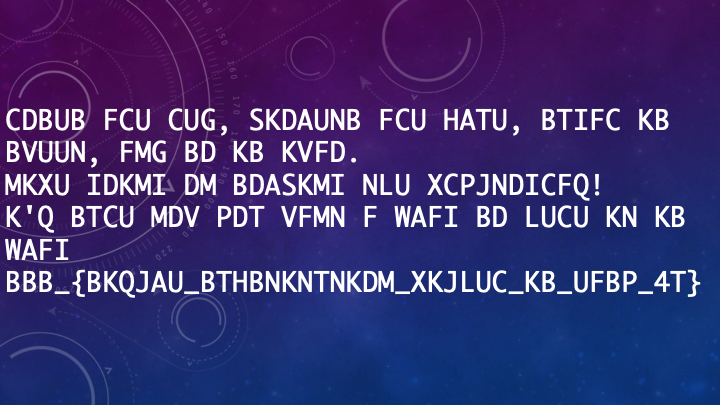
\includegraphics[clip, width=15.9cm]{./Challenge4.png}
	\end{center}
\end{figure}

\section{It's difficult to factorize the product of two large prime numbers (but I can do it in my head)}
\begin{figure}[H]
	\begin{center}
		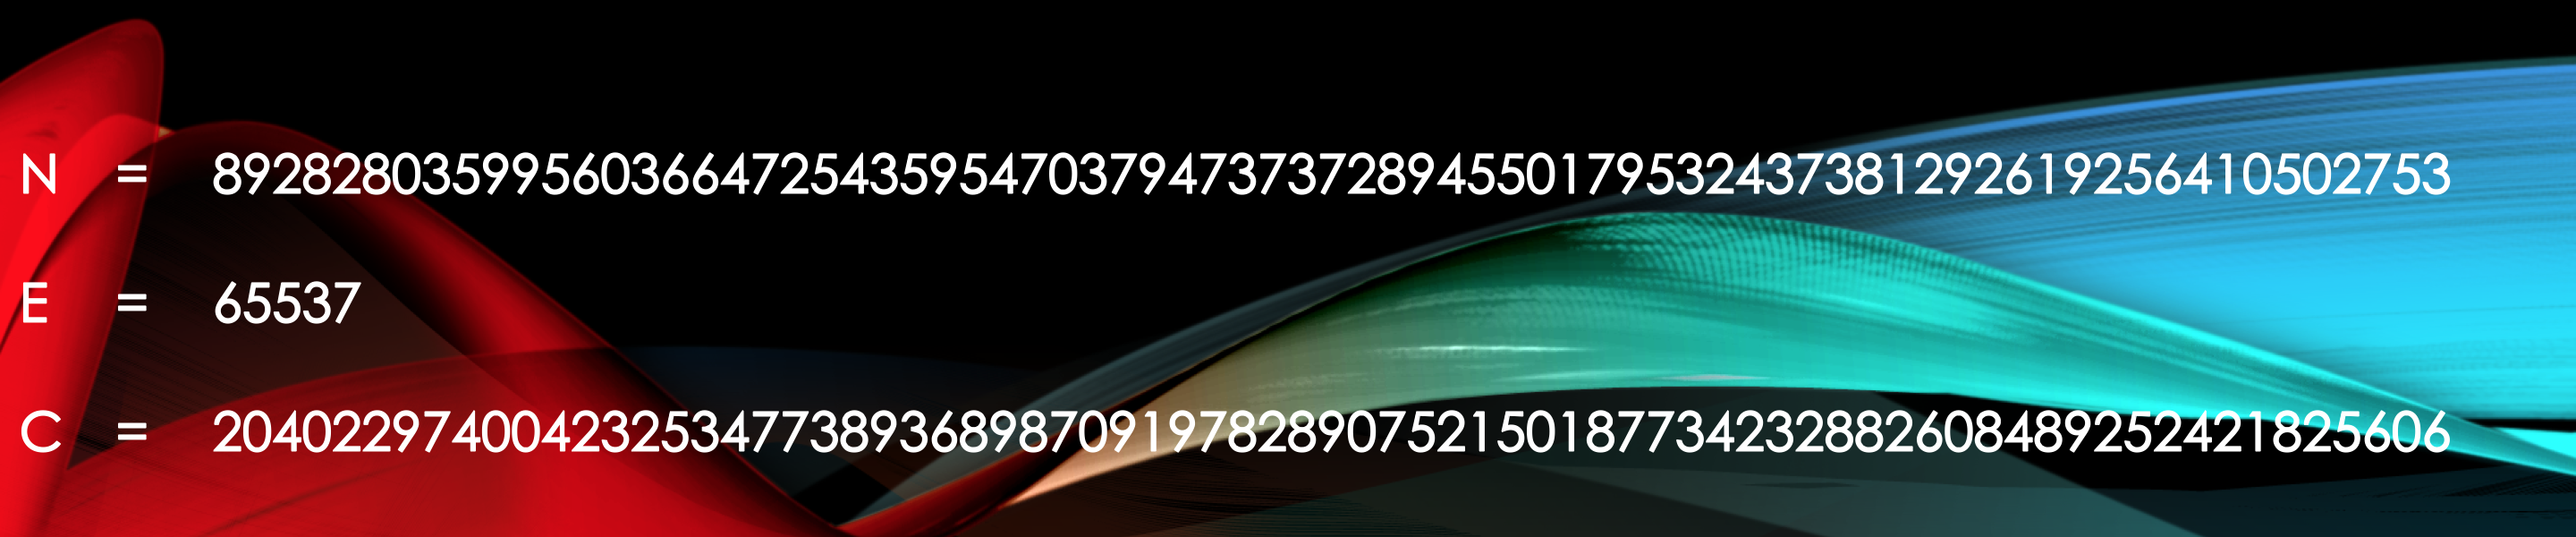
\includegraphics[clip, width=15.9cm]{./Challenge5.png}
	\end{center}
\end{figure}

\newpage

\textbf{Hints}
\setcounter{section}{0}

\section{I had rather be first in a village than second at Rome.}
\section{Japanese can't read this font.}
\section{School Days with a Pig}
\begin{figure}[H]
	\begin{center}
		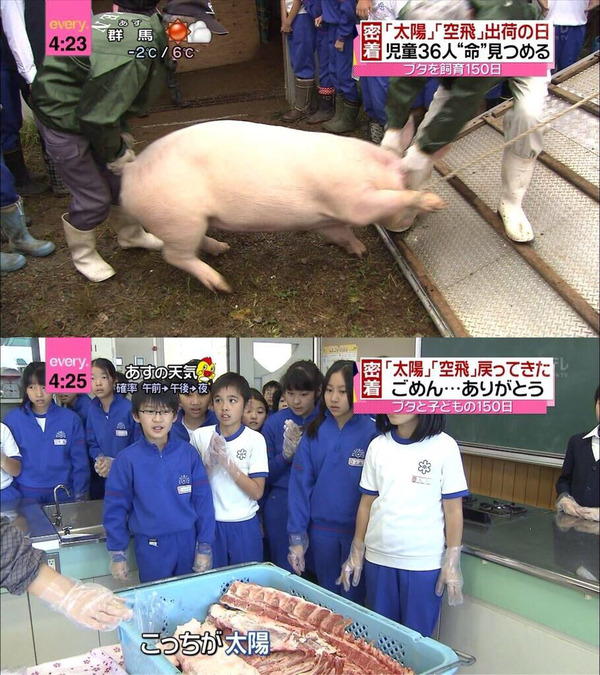
\includegraphics[clip, width=8.0cm]{./Hint3.jpg}
	\end{center}
\end{figure}

\section{B=S}
\section{msieve, Extended Euclidean Algorithm}

\end{document}
